\chapter*{ANEXO I - Teste de Integração Microsoft Power Automate}
\addcontentsline{toc}{chapter}{ANEXO I - Teste de Integração Microsoft Power Automate}
\label{anexoITIMPA}

Neste anexo, vamos descrever como realizar um teste de integração utilizando o Microsoft Power Automate para automatizar o envio de respostas de questionários para um ambiente externo.

\section*{Configurações Iniciais}

O primeiro passo é criar um fluxo na plataforma Microsoft Power Automate. Dentro do fluxo, siga as etapas abaixo:

\subsection*{1. Criar um novo fluxo}

Selecione a etapa \textbf{``Quando uma nova resposta é enviada''}.
Nesta etapa, vamos apenas selecionar o ID do questionário que desejamos observar.

\begin{figure}[H]
    \centering
    \caption{Etapa - Quando uma nova resposta é enviada}
    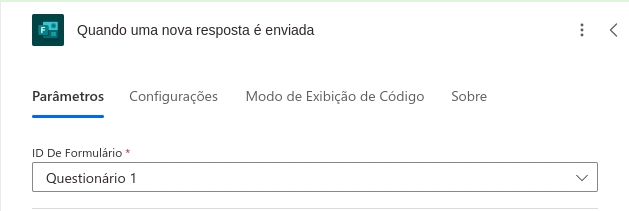
\includegraphics[width=1\textwidth]{figuras/mpa_new_answer.png}
    \label{fig:report_questions}
\end{figure}

\subsection*{2. Obter os detalhes da resposta}

Em seguida, selecione a etapa \textbf{``Obter os detalhes da resposta''}.
Aqui, vamos selecionar novamente o ID do questionário e o ID da resposta que queremos observar.

\begin{figure}[H]
    \centering
    \caption{Etapa - Obter os detalhes da resposta}
    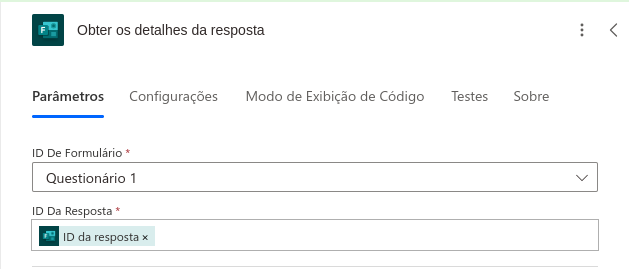
\includegraphics[width=1\textwidth]{figuras/mpa_detail_answer.png}
    \label{fig:report_questions}
\end{figure}

\subsection*{3. Realizar uma requisição HTTP}

A próxima etapa é adicionar o passo \textbf{``HTTP''}, que realizará uma requisição externa ao ambiente do Power Automate.
Como nossa API não está hospedada em nenhuma plataforma específica, vamos direcionar a requisição para o site \textbf{webhook.site}.
Este site permite monitorar todas as requisições externas que chegam a ele, exibindo o método utilizado, o payload, e todas as informações enviadas. Isso prova que é possível fazer uma requisição externa à plataforma.

\begin{figure}[H]
    \centering
    \caption{Etapa - HTTP}
    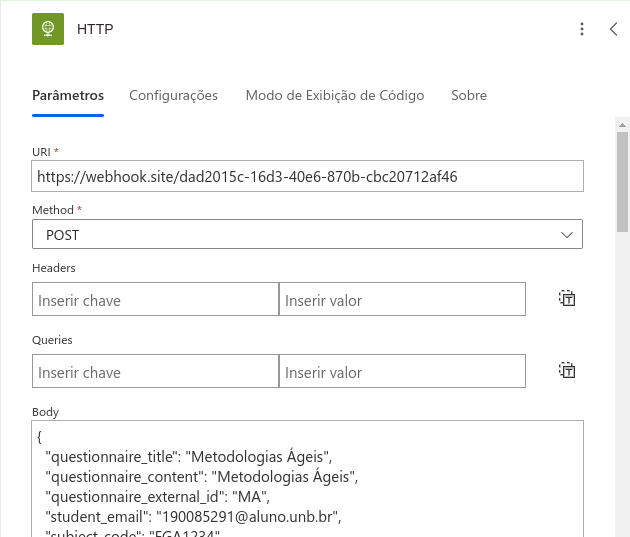
\includegraphics[width=1\textwidth]{figuras/mpa_http.png}
    \label{fig:report_questions}
\end{figure}

É possível automatizar as respostas dos usuários nos campos que serão enviados para a API utilizando o Power Automate, para isso só precisa ter selecionado corretamente o questionário desejado nos passos anteriores, e nessa etapa o próprio ambiente vai induzir ao usuário a selecionar os campos do questionário. 

Quando clicar no campo de texto nas configurações da requisição, o Power Automate vai exibir um ícone de raio, ao clicar nele, será possível visualizar uma lista com os campos do questionário, e o usuário pode selecionar os campos que deseja enviar para a API.

\begin{figure}[H]
    \centering
    \caption{Configurações das Respostas do Questionário}
    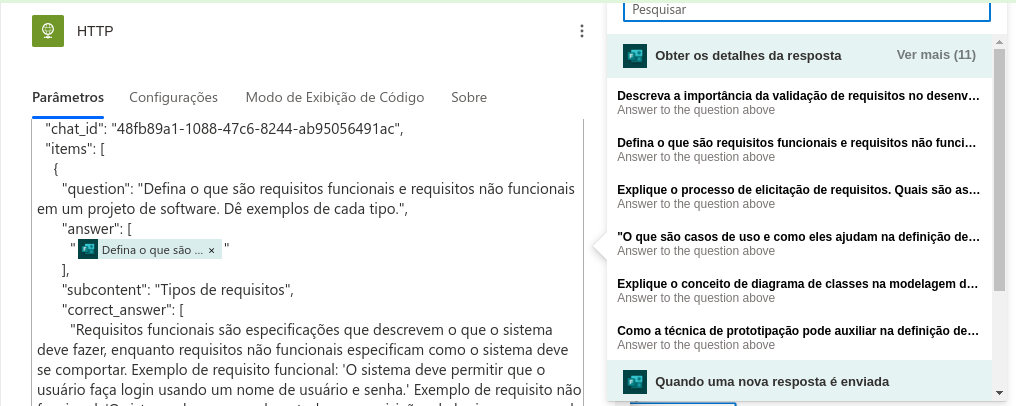
\includegraphics[width=1\textwidth]{figuras/mpa_example.png}
    \label{fig:report_questions}
\end{figure}

Podemos automatizar o envio das respostas e do e-mail dos estudantes, criando um payload que inclui todos esses dados. As perguntas, no entanto, devem ser adicionadas manualmente na configuração da requisição.

\subsection*{4. Testar o fluxo}

Com todas as etapas configuradas, é possível testar o fluxo. Para isso, basta enviar uma resposta para o questionário selecionado e verificar se a requisição foi enviada corretamente para o site \textbf{webhook.site}.

\begin{figure}[H]
    \centering
    \caption{Fluxo do Microsoft Power Automate}
    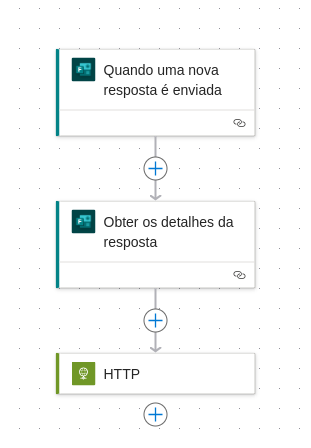
\includegraphics[width=1\textwidth]{figuras/mpa_geral_vision.png}
    \label{fig:report_questions}
\end{figure}

\begin{figure}[H]
    \centering
    \caption{Requisição enviada para o site webhook.site - Detalhes da Requisição e Headers}
    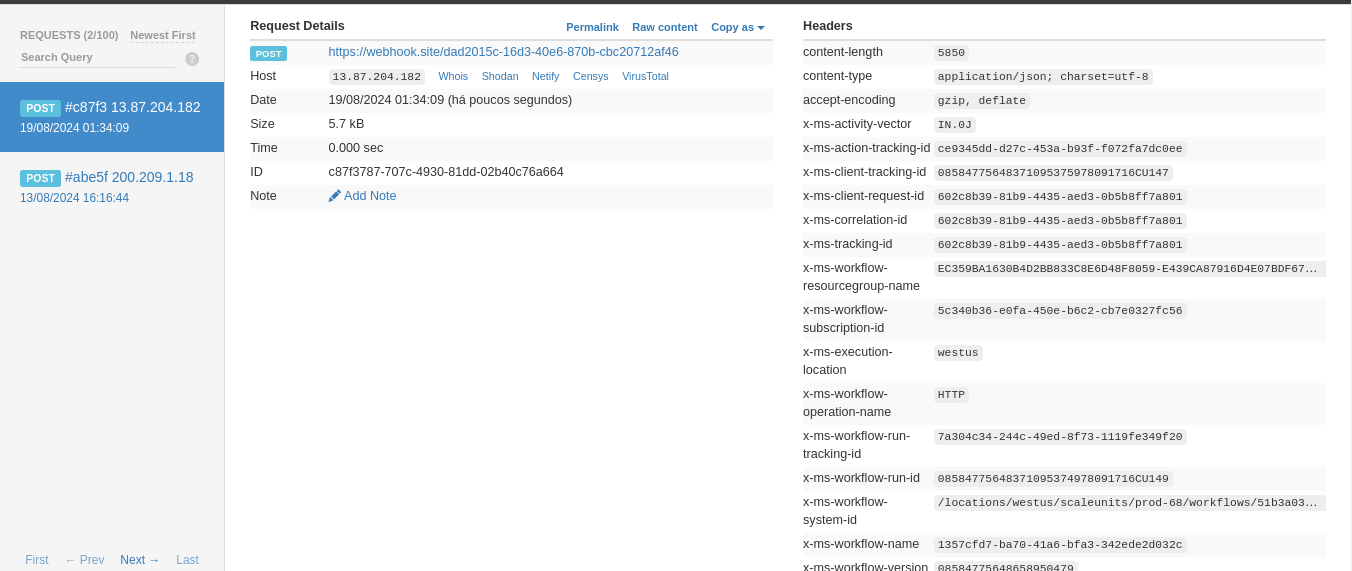
\includegraphics[width=1\textwidth]{figuras/webhook_1.png}
    \label{fig:report_questions}
\end{figure}

\begin{figure}[H]
    \centering
    \caption{Requisição enviada para o site webhook.site - Body da Requisição}
    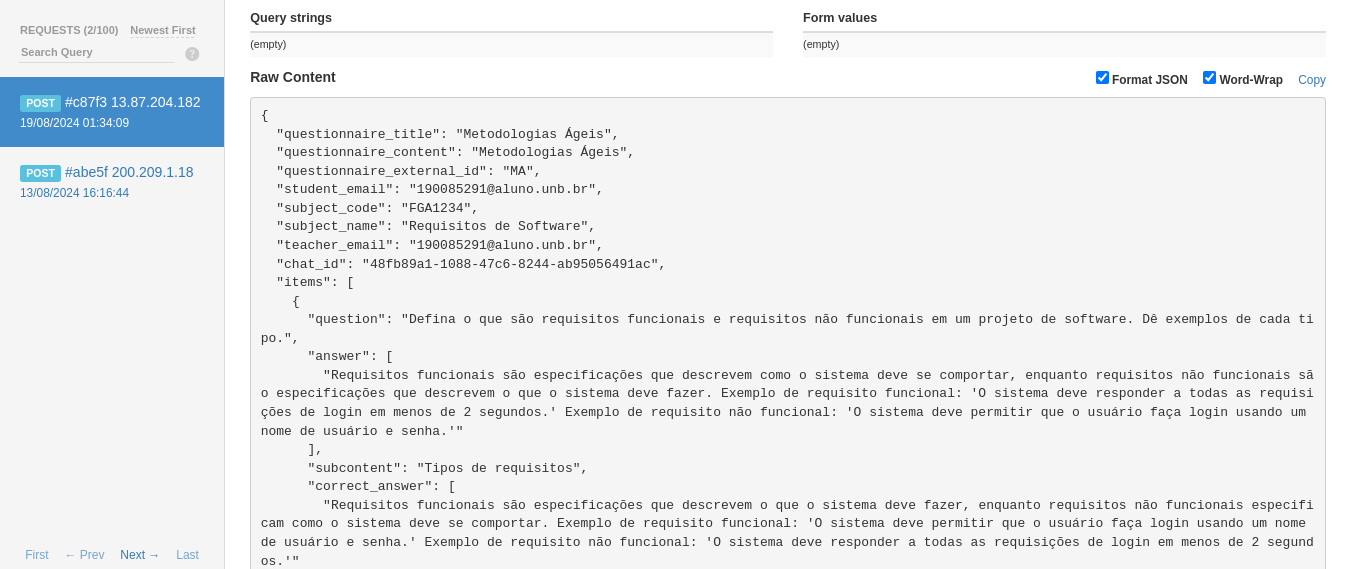
\includegraphics[width=1\textwidth]{figuras/webhook_2.png}
    \label{fig:report_questions}
\end{figure}

Por fim, basta copiar os dados da requisição e enviá-los para a API desejada para comprovar o funcionamento do fluxo.